\secrel{Библиотеки компонентов}\secdown

\cp{http://habrahabr.ru/post/197582/}\bigskip

Модель компонента в САПР EDA состоит из следующих частей:

\begin{itemize}
  \item условное графическое обозначение (УГО) для схемного редактора
  \item модель компонента для редактора печатных плат (ПП)
  \item модель для симулятора (SPICE)
  \item 3D модель для передачи в универсальный САПР для работы с конструкцией
  \item дополнительные пользовательские данные: индексы компонента для
  заказа у разных поставщиков, ссылки на документацию, и т.п.
\end{itemize}

Части могут иметь несколько вариантов, например два варианта УГО (ГОСТ и ISO),
три корпуса (DIP, PLCC и LQFP), две модели для симулятора (идеальная и с
учетом паразитных эффектов), и 2 механических модели (габаритный кубик, и
подробная).

Кроме того, часто в один корпус упаковывается несколько одинаковых или разных
элементов. Одинаковые\ --- 2--4 операционных усилителя (ОУ), или вентили
логики. Разные\ --- части вакуумной лампы, разнесенные на схеме по разным
каскадам.

\bigskip

В составе KiCad поставляются библиотеки электронных компонентов (обычных и
поверхностно монтируемых SMD). Для многих библиотечных компонентов есть
3D-модели, созданные в \prog{Wings3D}.

Но как только вы начинаете работать со свежеустановленным KiCADом, тут же
обнаруживается, что библиотечные компоненты или не подходят\note{например не
соответствуют ГОСТ или стандартам предприятия}, или нужных компонентов попросту
нет в библиотеках.

Рассмотрим последовательное создание совершенно нового элемента на примере
модуля USB интерфейса HEX\_FT2232RL \ref{HEXFT2232RL}

\secrel{Создание УГО для схем}

Нам необходим встроенный редактор символов схем (библиотечных компонентов),
запускаем его следующим образом:

\begin{enumerate}
  \item Вначале запускаем \file{eeschema}
  \begin{itemize}
    \item[вверху] меню и панель инструментов
    \item[слева] область размерности и шага сетки редактора (настройка рабочей
    области)
    \item[справа] область элементов схем и перемещения по иерархии схемы
  \end{itemize}
  \item Далее запускаем встроенный
  \menu{Редактор библиотек}\ 
\includegraphics[height=2em]{kicad/ee22.png}

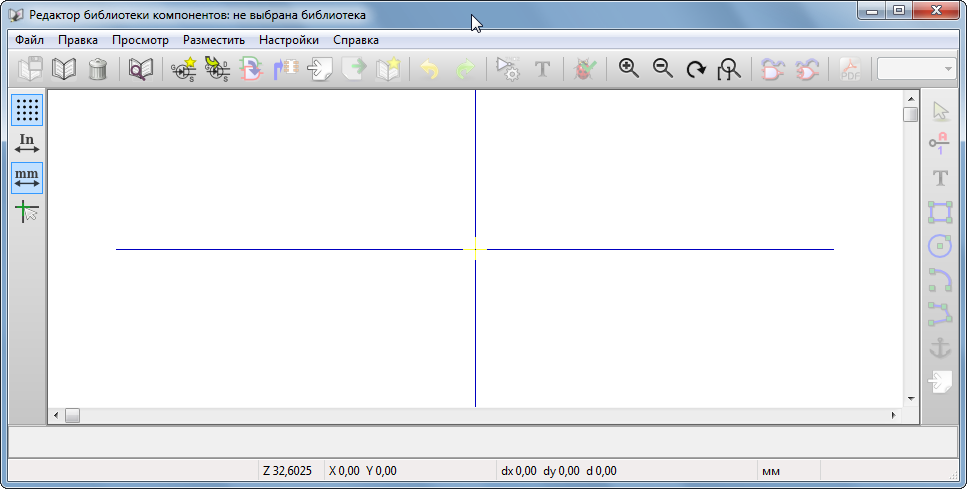
\includegraphics[height=0.5\textheight]{kicad/lib23.png}
\end{enumerate}

Необходимо создать новую библиотеку и первый собственный компонент:

\menu{Создать новый компонент}
\includegraphics[height=2em]{kicad/newel.png},

\menu{Свойства компонента>Общие Настройки},

\menu{Имя компонента>HEX\_FT232RL}

\menu{Обозначение по умолчанию>U}

\menu{Количество элементов в корпусе>1}

\menu{OK}
\bigskip

В верхней панели инструментов активировались несколько кнопок, выбираем

\menu{Сохранить текущий компонент в новой библиотеке}

\includegraphics[height=2em]{kicad/lib26.png}

В открывшемся диалоге выберите каталог для библиотеки
\file{/home/user/kicad/}, и укажите имя файла (новой) библиотеки
\menu{\file{MyModules}>Сохранить}.

\bigskip
Теперь нужно добавить созданную библиотеку в рабочий список.
\bigskip

Настроим дополнительный путь, где лежат файлы библиотек. Это могут быть ваши
личные библиотеки, специальная библиотека для конкретного проекта, или комплект
библиотек поставляемых вместе с этой книгой: выберите в меню
\menu{Настройки>Библиотека}, \menu{Пользовательские пути
поиска>добавить>\file{/home/user/kicad/}}, \menu{Ok}.

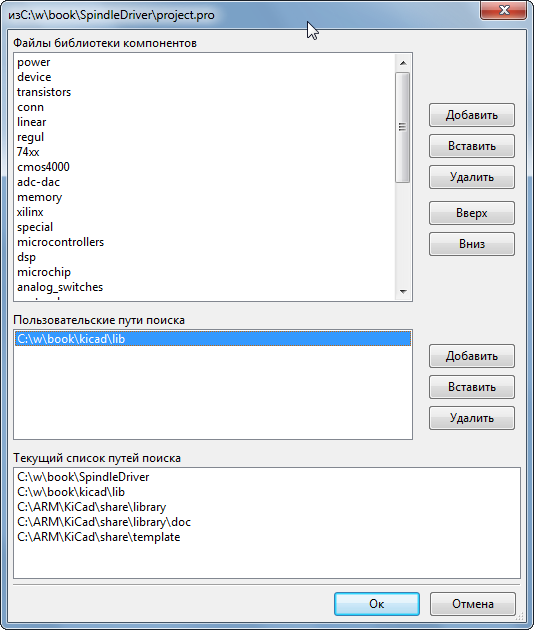
\includegraphics[height=0.5\textheight]{kicad/lib25.png}

\menu{Настройки>Библиотека},
\menu{Файлы библиотеки компонентов>power>\lms>Вставить}.
Выбираем только что созданную библиотеку \file{MyModules}.
Она будет вставлена в список до выбранной \file{power}.

\bigskip
Проделанные настройки применятся только к текущему проекту. Если Вы хотите 
чтобы новая библиотека всегда добавлялась к новым проектам, вам нужно добавить
новый путь поиска библиотек и ее название в файл шаблона, как это описано в
\ref{kicadtemplates}.

\bigskip
Если вы хотите изменить только что созданное или уже сущесствующее УГО, нужно
выбрать рабочую библиотеку, ту библиотеку в которой мы хотим работать (создавать
или редактировать компоненты). На панели инструментов нажимается кнопка

\menu{Выбор рабочей библиотеки}
\includegraphics[height=2em]{kicad/lib24.png},

\menu{Выбрать библиотеку>MyModules>Ok}.

Загружаем созданный ранее (пустой) компонент \file{HEX\_FT232RL} (или любой
другой)

\menu{Загрузить компонент для редактирования}

\includegraphics[height=2em]{kicad/editel.png}

\menu{Выбор компонента>Список всех>Элементы>\file{HEX\_FT232RL}>Ok}

\bigskip
\includegraphics[height=0.45\textheight]{odurino/usb/HEXFT232RL.png}

Сейчас у нас элемент не имеет графических элементов, и состоит только из
нескольких текстовых полей с обозначениями, слепленных в одной точке. Нужно их
растащить: \rms, САПР не может различить близкие элементы и уточняет для
какого поля мы хотим контекстное меню. Выбираем любое, \menu{Переместить поле}\
или кнопка \keys{M}. Перетаскиваем элемент, и \lms\ на свободном месте.

Пользуясь \ref{eskd}, отрисовываем на освободившемся месте УГО элемента,
пользуясь кнопками на панели справа. Рисование выполняется по сетке, шаг
выбирается \menu{\rms>Выбор сетки}, набор сеток фиксированный (?). При рисовании
ГОСТовских УГО округляем до ближайших дюймовых размеров\footnote{\ 1mil=1/1000
дюйма, 100mil=2.54mm=типовой шаг DIP микросхем}, или в меньшей сетке если нужно
точно гостовские размеры.

УГО имеет \term{точку привязки}, относительно которой отрисовываются элементы.
На практике важно то, что вокруг этой точки элемент вращается. Для перемещения
этой точки можно использовать кнопку

\menu{Переместить точку привязки}
\includegraphics[height=2em]{kicad/lib27.png}.

Добавляем выводы компонента: \menu{Добавить вывод
компонента}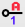
\includegraphics[height=2em]{kicad/lib28.png}.

\bigskip
Например для резистора создание выводов будет выглядеть вот так:

\bigskip
\menu{Свойства вывода}

\menu{Имя>A}

\menu{Номер>1}

\menu{Ориентация>Вправо}

\menu{Электр.тип>Пассивный}

\menu{Размер шрифта>1.27мм}

\menu{Длина>2.54мм}

\menu{Ok}

\bigskip

\menu{Имя>B}

\menu{Номер>2}

\menu{Ориентация>Влево}

\menu{Ok}

\bigskip
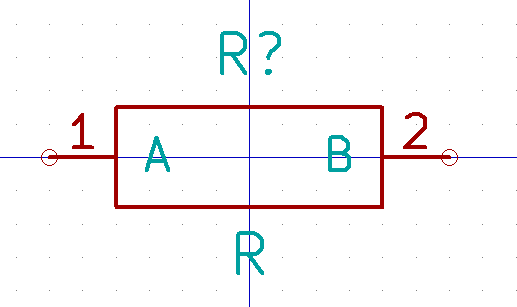
\includegraphics[height=0.5\textheight]{kicad/lib29.png}
\bigskip

Сохраняем библиотеку: \menu{Сохранить текущую
библиотеку}
\includegraphics[height=2em]{kicad/lib30.png}

\menu{Подтверждение>Включая последние изменения компонента?>Да}

\menu{Подтверждение>Компонент существует. Изменить его?>Да}

\menu{Подтверждение>Изменить файл библиотеки ?>Да}

\secrel{Создание падстека}

% \secrel{PS:}
% 
% Компоненты и посадочные места корпусов можно ассоциировать с документацией,
% ключевыми словами и осуществлять быстрый поиск компонента по функциональному
% назначению.
% 
% \secup
% 
% \secru{Отрисовка схемы (часть 2)}
% 
% \secdown
% 
% \secru{Автоматическое обозначение элементов}
% 
% Автоматическое обозначение элементов и перенумерация выполняется кнопкой\\
% \menu{Обозначить компоненты на
% схеме}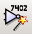
\includegraphics[height=2em]{kicad/ee000004.png}
% 
% \secru{Генерация списка цепей}
% 
% Список цепей (нетлист) используется для передачи информации о соединении
% компонентов между программами. Чаще всего СЦ создается после отрисовки схемы для
% передачи данных в программу трассировки печатной платы (ПП).

\secup
